\chapter{Kiến trúc hệ thống}
\label{ch:phuong-phap-de-xuat}

\section{Tổng quan kiến trúc hệ thống}

\subsection{Mục tiêu kiến trúc}
Kiến trúc của hệ thống Student360 được thiết kế nhằm đạt được bốn mục tiêu chính: (1) phân tách rõ ràng trách nhiệm giữa các thành phần (Separation of Concerns), giúp mỗi phần chỉ tập trung xử lý đúng vai trò của mình; (2) cho phép các thành phần được phát triển, kiểm thử và vận hành độc lập với nhau; (3) hỗ trợ nhiều thành viên trong nhóm phát triển song song trên các phần khác nhau của hệ thống mà không xung đột mã nguồn với nhau, phù hợp với cách phân công theo cặp đã trình bày ở Chương 5; (4) cô lập được rủi ro và chi phí vận hành của thành phần Trí tuệ nhân tạo (độ trễ, chi phí gọi mô hình ngôn ngữ lớn) khỏi luồng nghiệp vụ lõi của hệ thống.

\subsection{Mô hình kiến trúc tổng thể}
Hệ thống được tổ chức theo mô hình \textbf{Kiến trúc Client--Server phân tán nhiều tầng}, gồm ba tầng logic: tầng trình bày (Presentation Tier), tầng ứng dụng/xử lý nghiệp vụ (Application Tier) và tầng dữ liệu (Data Tier). Về mặt triển khai mã nguồn, mỗi thành phần thuộc tầng trình bày và tầng ứng dụng được hiện thực trong một repository Git độc lập (đa-repository), không dùng chung một repository duy nhất. Các thành phần giao tiếp với nhau hoàn toàn qua mạng, thông qua các giao thức kết nối tiêu chuẩn như HTTP REST, Server-Sent Events (SSE) và hàng đợi thông điệp (Message Queue), chứ không chia sẻ trực tiếp mã nguồn hay tiến trình với nhau. Cách tổ chức này cho phép mỗi dịch vụ được phát triển, triển khai và mở rộng độc lập, đồng thời phù hợp với quy mô một nhóm nhỏ (6 thành viên) khi mỗi cặp thành viên có thể làm việc trọn vẹn trên repository của mình mà ít va chạm với phần việc của cặp khác.

\subsection{Các thành phần chính và vai trò}
\begin{itemize}
    \item \textbf{Mobile App:} Kênh tương tác chính của sinh viên với hệ thống, thuộc tầng trình bày.
    \item \textbf{Web Admin Portal:} Công cụ quản trị dành cho nhà tài trợ và quản trị viên, thuộc tầng trình bày.
    \item \textbf{Backend:} Trung tâm xử lý nghiệp vụ, xác thực, phân quyền và điều phối truy cập dữ liệu, thuộc tầng ứng dụng.
    \item \textbf{AI Service:} Dịch vụ chuyên trách xử lý ngôn ngữ tự nhiên và các tác vụ liên quan tới Trí tuệ nhân tạo, thuộc tầng ứng dụng.
    \item \textbf{Tầng lưu trữ (PostgreSQL và Redis):} Nơi lưu trữ dữ liệu nghiệp vụ và quản lý hàng đợi xử lý bất đồng bộ, thuộc tầng dữ liệu.
\end{itemize}

Hình~\ref{fig:context-diagram} mô tả sơ đồ ngữ cảnh hệ thống (System Context Diagram), thể hiện các tác nhân tương tác với hệ thống và các hệ thống bên ngoài mà Student360 phụ thuộc vào.

\begin{figure}[H]
    \centering
    \begin{tikzpicture}[
        node distance=1.1cm and 2.6cm,
        actor/.style={draw, rounded corners, minimum width=3cm, minimum height=1.05cm, align=center, fill=blue!8, font=\small},
        system/.style={draw, thick, rounded corners, minimum width=4cm, minimum height=4.6cm, align=center, fill=blue!15, font=\small},
        ext/.style={draw, rounded corners, minimum width=3.3cm, minimum height=1.05cm, align=center, fill=gray!12, font=\small},
        lbl/.style={font=\tiny, align=center}
    ]
        \node[system] (sys) {\shortstack{\textbf{Hệ thống Student360}\\[3pt]\footnotesize Quản lý tài chính,\\học bổng và học thuật\\cho sinh viên}};

        \node[actor, left=of sys, yshift=1.7cm] (sv) {Sinh viên};
        \node[actor, left=of sys] (nt) {Nhà tài trợ};
        \node[actor, left=of sys, yshift=-1.7cm] (qt) {Quản trị viên};

        \node[ext, right=of sys, yshift=1.4cm] (llm) {\shortstack{Nhà cung cấp\\Mô hình ngôn ngữ lớn}};
        \node[ext, right=of sys, yshift=-1.4cm] (fcm) {\shortstack{Firebase Cloud\\Messaging}};

        \draw[->] (sv) -- node[lbl, above] {Ghi nhận chi tiêu, trò chuyện AI} (sys.west |- sv);
        \draw[->] (nt) -- node[lbl, above] {Đăng và duyệt học bổng} (sys.west |- nt);
        \draw[->] (qt) -- node[lbl, below] {Quản trị dữ liệu học thuật} (sys.west |- qt);

        \draw[->] (sys.east |- llm) -- node[lbl, above] {Yêu cầu suy luận ngôn ngữ tự nhiên} (llm);
        \draw[->] (sys.east |- fcm) -- node[lbl, below] {Gửi thông báo đẩy} (fcm);
    \end{tikzpicture}
    \caption{Sơ đồ ngữ cảnh hệ thống (System Context Diagram) của Student360}
    \label{fig:context-diagram}
\end{figure}

Ở mức chi tiết hơn, Hình~\ref{fig:container-diagram} trình bày sơ đồ kiến trúc Container, thể hiện các thành phần triển khai cụ thể (Mobile App, Web Admin Portal, Backend, AI Service, hàng đợi và tầng lưu trữ) cùng giao thức giao tiếp giữa chúng.

\begin{figure}[H]
    \centering
    
\includegraphics[width=\linewidth]{fig3_1_monorepo.png}
    \caption{Sơ đồ kiến trúc Container của hệ thống Student360}
    \label{fig:container-diagram}
\end{figure}

\subsection{Luồng hoạt động tổng quát}
Người dùng thao tác trên Mobile App hoặc Web Admin Portal, gửi yêu cầu tới Backend qua giao thức HTTP REST thông thường, hoặc qua kênh SSE riêng đối với chức năng trò chuyện AI cần phản hồi theo thời gian thực. Backend xác thực danh tính và phân quyền truy cập, sau đó xử lý nghiệp vụ và đọc/ghi dữ liệu trực tiếp trên PostgreSQL. Đối với các yêu cầu cần năng lực xử lý ngôn ngữ tự nhiên (tư vấn tài chính, phân loại giao dịch, gợi ý học bổng), Backend đóng vai trò cổng trung gian, chuyển tiếp yêu cầu sang AI Service; AI Service không truy cập trực tiếp vào cơ sở dữ liệu mà luôn gọi ngược lại Backend để lấy dữ liệu thật khi cần suy luận. Kết quả xử lý cuối cùng được trả ngược qua Backend về lại giao diện người dùng. Đối với các tác vụ không cần phản hồi tức thời (gửi thông báo hàng loạt, xử lý nền định kỳ), Backend đẩy tác vụ vào hàng đợi Redis để xử lý bất đồng bộ, tránh làm chậm các yêu cầu API chính.

\section{Kiến trúc Frontend}

\subsection{Ứng dụng Mobile}
Ứng dụng Mobile (Expo/React Native) là kênh tương tác chính của sinh viên với hệ thống, đảm nhận việc ghi nhận thu chi tài chính, trò chuyện với trợ lý AI, ứng tuyển học bổng, quản lý bảng điểm cá nhân và nhận thông báo đẩy.

Về mặt tổ chức, ứng dụng được chia thành ba tầng logic tách biệt: tầng giao diện và định tuyến, tổ chức theo mô hình định tuyến dựa trên tệp tin (file-based routing) giúp cấu trúc màn hình phản ánh trực tiếp cấu trúc điều hướng của ứng dụng; tầng trạng thái, tách biệt rõ giữa trạng thái phiên đăng nhập/giao diện cục bộ và trạng thái dữ liệu nghiệp vụ được đồng bộ từ máy chủ; và tầng giao tiếp API, tập trung toàn bộ việc gọi Backend qua một lớp client duy nhất.

Về xử lý dữ liệu, trạng thái phiên đăng nhập và các trạng thái giao diện cục bộ (như phiên trò chuyện AI, bộ lọc hiển thị) được quản lý độc lập với trạng thái dữ liệu nghiệp vụ lấy từ Backend. Dữ liệu nghiệp vụ được đồng bộ hai chiều với Backend thông qua cơ chế làm mới bộ đệm tự động mỗi khi có thay đổi (đã trình bày cơ chế cụ thể ở Chương 6, mục Cơ chế đồng bộ trạng thái giao diện tức thời), giúp số dư và lịch sử giao dịch trên màn hình luôn phản ánh đúng dữ liệu mới nhất mà không cần người dùng tải lại thủ công. Lớp giao tiếp API tự động đính kèm token xác thực vào mỗi yêu cầu và tự động làm mới token khi hết hạn, giúp phiên đăng nhập của người dùng được duy trì liền mạch.

Việc lựa chọn nền tảng Expo/React Native cho phép phát triển đồng thời cho cả iOS và Android từ một mã nguồn duy nhất, phù hợp với quy mô và thời gian phát triển hạn chế của một đồ án tốt nghiệp. Thư viện thiết kế giao diện Tamagui được sử dụng nhất quán trong toàn bộ ứng dụng, đảm bảo giao diện đồng bộ về phong cách và tối ưu về hiệu năng hiển thị trên thiết bị di động.

\subsection{Web Admin}
Web Admin Portal (React JS/Vite) là công cụ dành cho quản trị viên và nhà tài trợ, phục vụ việc quản lý dữ liệu học thuật chuẩn hóa (trường, chương trình đào tạo, môn học) và toàn bộ vòng đời của một chương trình học bổng, từ khởi tạo, cấu hình điều kiện cho tới xét duyệt hồ sơ ứng tuyển của sinh viên.

Về mặt tổ chức, Web Admin Portal được chia theo miền nghiệp vụ, mỗi miền là một khối chức năng độc lập có luồng dữ liệu và giao diện riêng. Việc kiểm soát truy cập theo vai trò (quản trị viên hay nhà tài trợ) được thực hiện ngay ở tầng định tuyến, đảm bảo mỗi vai trò chỉ nhìn thấy và thao tác được trên đúng phần giao diện được phép truy cập.

Trạng thái đăng nhập và thông tin phân quyền của người dùng được quản lý tập trung trong toàn ứng dụng, trong khi dữ liệu nghiệp vụ của từng miền chức năng (danh sách trường, danh sách học bổng, hồ sơ ứng tuyển...) được đồng bộ riêng theo từng khu vực giao diện tương ứng. Giống như ứng dụng Mobile, Web Admin Portal giao tiếp với Backend qua một lớp client tập trung, tự động đính kèm token xác thực vào mỗi yêu cầu.

Việc lựa chọn React JS kết hợp Vite giúp tối ưu tốc độ phát triển và build ứng dụng, trong khi thư viện Material UI cho phép dựng nhanh các giao diện quản trị dữ liệu dạng bảng với khối lượng bản ghi lớn, vốn là nhu cầu chính của một cổng quản trị.

\section{Kiến trúc Backend}

\subsection{Vai trò}
Backend, hiện thực trên nền tảng NestJS \cite{nestjs-docs}, là trung tâm điều phối của toàn hệ thống: xác thực người dùng, phân quyền truy cập, xử lý toàn bộ logic nghiệp vụ, là điểm truy cập duy nhất tới cơ sở dữ liệu quan hệ, đồng thời đóng vai trò cổng trung gian (gateway) an toàn cho các yêu cầu cần tới năng lực xử lý của AI Service. Việc lựa chọn NestJS xuất phát từ kiến trúc module hóa sẵn có của framework (hỗ trợ tách rời Controller, Service và Guard một cách tường minh, phù hợp trực tiếp với mô hình phân lớp trình bày ở Mục 3.3.2) và hệ sinh thái TypeScript giúp giảm thiểu lỗi thời gian chạy khi nhiều thành viên cùng phát triển song song trên các module khác nhau.

\subsection{Mô hình kiến trúc}
Backend được tổ chức theo \textbf{Kiến trúc phân lớp (Layered Architecture)}: một dịch vụ duy nhất, được module hóa rõ ràng theo từng miền nghiệp vụ, chứ không tách thành nhiều dịch vụ vận hành độc lập theo đúng nghĩa Microservices, cũng không áp dụng các mô hình như CQRS (tách biệt luồng xử lý lệnh ghi và truy vấn đọc) hay kiến trúc hướng sự kiện (Event-driven Architecture) với cơ chế phát/nhận sự kiện nghiệp vụ. Lựa chọn này xuất phát từ quy mô của nhóm phát triển (6 thành viên) và thời gian thực hiện đồ án có giới hạn: việc module hóa theo miền nghiệp vụ trong một dịch vụ duy nhất đã đủ để tách biệt rõ trách nhiệm giữa các phần chức năng, trong khi tránh được chi phí vận hành và điều phối phát sinh khi phải triển khai, giám sát và đồng bộ dữ liệu giữa nhiều dịch vụ độc lập như kiến trúc Microservices thực thụ đòi hỏi.

\subsection{Các tầng nội bộ}
Một yêu cầu đi qua Backend lần lượt qua các tầng sau:
\begin{itemize}
    \item \textbf{Tầng tiếp nhận và xác thực yêu cầu:} tiếp nhận yêu cầu từ client, xác thực danh tính người dùng qua JSON Web Token (JWT) và kiểm tra quyền truy cập theo vai trò trước khi cho phép yêu cầu đi tiếp.
    \item \textbf{Tầng chuẩn hóa và giám sát:} chuẩn hóa cấu trúc phản hồi trả về và ghi log của mỗi yêu cầu, phục vụ việc theo dõi và gỡ lỗi hệ thống.
    \item \textbf{Tầng xử lý nghiệp vụ:} nơi hiện thực toàn bộ logic nghiệp vụ cốt lõi của hệ thống, độc lập với cách yêu cầu được tiếp nhận hay dữ liệu được lưu trữ.
    \item \textbf{Tầng truy xuất dữ liệu:} chịu trách nhiệm đọc/ghi dữ liệu trên PostgreSQL, cô lập tầng xử lý nghiệp vụ khỏi chi tiết truy vấn cơ sở dữ liệu.
    \item \textbf{Tầng đẩy tác vụ nền:} đối với các tác vụ không cần phản hồi tức thời (gửi thông báo hàng loạt, lên lịch giao dịch định kỳ), Backend đẩy tác vụ vào hàng đợi Redis/BullMQ thay vì xử lý đồng bộ trong cùng một yêu cầu, giúp không làm chậm tiến trình xử lý API chính.
\end{itemize}

\subsection{Tổ chức theo miền nghiệp vụ}
Trong phạm vi đề tài này, Backend được tổ chức thành các miền nghiệp vụ chính: Xác thực và phân quyền, Tài chính 6 lọ, Học bổng, Học thuật/Bảng điểm và Thông báo. Cần lưu ý rằng Backend là nền tảng dùng chung cho toàn bộ hệ sinh thái Student360, phục vụ cả các phân hệ khác ngoài phạm vi đồ án này; nội dung trình bày trong báo cáo chỉ tập trung vào các miền nghiệp vụ liên quan trực tiếp tới tài chính, học bổng và học thuật.

\subsection{Nguyên tắc thiết kế áp dụng}
\begin{itemize}
    \item \textbf{Phân tách trách nhiệm:} tầng xác thực/phân quyền và tầng chuẩn hóa phản hồi được tách hoàn toàn khỏi tầng xử lý nghiệp vụ, mỗi thay đổi về quy tắc xác thực hay định dạng phản hồi không ảnh hưởng tới logic nghiệp vụ.
    \item \textbf{Khả năng mở rộng:} việc module hóa theo miền nghiệp vụ cho phép bổ sung miền chức năng mới mà không ảnh hưởng tới các miền đã có; xử lý bất đồng bộ qua hàng đợi giúp hệ thống chịu tải tốt hơn khi cần gửi thông báo tới số lượng lớn người dùng cùng lúc.
    \item \textbf{Khả năng bảo trì:} cấu trúc module hóa rõ ràng theo miền nghiệp vụ giúp việc định vị và sửa lỗi trong một miền cụ thể không đòi hỏi phải hiểu toàn bộ hệ thống.
    \item \textbf{Khả năng tích hợp hệ thống ngoài:} việc gọi sang AI Service được cô lập qua một lớp client HTTP trung gian riêng biệt, giúp phần lõi nghiệp vụ của Backend không phụ thuộc trực tiếp vào chi tiết triển khai của AI Service, dễ dàng thay đổi hoặc nâng cấp AI Service mà không ảnh hưởng Backend.
\end{itemize}

\section{Kiến trúc hệ thống AI}

\subsection{Vai trò và vị trí trong kiến trúc tổng thể}
AI Service, hiện thực bằng FastAPI \cite{fastapi-docs} kết hợp thư viện LangChain \cite{langchain-docs} để xây dựng tác nhân AI và kết nối tới mô hình ngôn ngữ lớn Gemini \cite{gemini-api} của Google, cung cấp năng lực xử lý ngôn ngữ tự nhiên cho hệ thống: tư vấn tài chính qua hội thoại, phân loại giao dịch từ mô tả viết tay của người dùng, và gợi ý học bổng phù hợp với hồ sơ sinh viên. Dịch vụ này được tách thành một thành phần độc lập trong kiến trúc tổng thể nhằm cô lập độ trễ và chi phí gọi mô hình ngôn ngữ lớn khỏi luồng xử lý nghiệp vụ lõi của Backend. AI Service chỉ tiếp nhận yêu cầu từ Backend, không có client nào được phép gọi trực tiếp; mọi yêu cầu giữa hai dịch vụ đều được xác thực nội bộ bằng một token dùng chung. Việc lựa chọn Python/FastAPI thay vì cùng nền tảng NestJS với Backend xuất phát từ hệ sinh thái thư viện AI/LLM phong phú của Python, trong khi LangChain cung cấp sẵn các thành phần trừu tượng hóa cho tác nhân tool-calling và khả năng tích hợp đa nhà cung cấp mô hình ngôn ngữ, phù hợp trực tiếp với tầng trừu tượng hóa LLM mô tả ở Mục 3.4.3.

\subsection{Luồng xử lý tổng quát}
Khi sinh viên đặt một câu hỏi hoặc nhập một mô tả giao dịch trên Mobile App, yêu cầu được Backend xác thực rồi chuyển tiếp sang AI Service. Tại đây, hệ thống trước tiên phân loại ý định của câu hỏi để xác định ngữ cảnh và phạm vi xử lý phù hợp, sau đó một tác nhân AI (Agent) tiến hành suy luận theo mô hình lặp truy vấn--hành động (ReAct: reasoning + acting) \cite{yao2022-react}, gọi tới các công cụ nghiệp vụ tương ứng khi cần dữ liệu thực tế (thông qua việc gọi ngược lại Backend). Kết quả sau khi được tổng hợp từ mô hình ngôn ngữ lớn được trả về dưới dạng luồng token liên tục cho Backend, và Backend tiếp tục đẩy luồng này về ứng dụng di động để hiển thị theo thời gian thực, tương tự trải nghiệm của các trợ lý ảo thương mại.

\subsection{Các thành phần chính}
\begin{itemize}
    \item \textbf{Tầng tiếp nhận yêu cầu:} nhận yêu cầu từ Backend, xác thực token nội bộ trước khi chuyển tiếp cho tầng xử lý.
    \item \textbf{Tầng phân loại ý định:} xác định loại câu hỏi (truy vấn tài chính, phân loại giao dịch, tư vấn học bổng...) để giới hạn đúng phạm vi ngữ cảnh và tập công cụ được phép sử dụng cho từng loại câu hỏi, thay vì luôn cho phép toàn bộ công cụ có sẵn -- giúp giảm chi phí gọi mô hình và tăng độ chính xác của kết quả.
    \item \textbf{Tầng suy luận và gọi công cụ:} một tác nhân AI duy nhất theo mô hình tool-calling (ReAct), được "thu hẹp phạm vi" linh hoạt theo kết quả phân loại ý định ở bước trước, thay vì cần nhiều tác nhân chuyên biệt tách rời phối hợp với nhau.
    \item \textbf{Tầng công cụ nghiệp vụ:} tập hợp các hàm truy vấn và tính toán cụ thể mà tác nhân AI có thể gọi khi cần dữ liệu thực tế, ví dụ truy vấn số dư hũ tài chính, lịch sử giao dịch, hoặc tính điểm phù hợp giữa hồ sơ sinh viên và một chương trình học bổng.
    \item \textbf{Tầng trừu tượng hóa nhà cung cấp mô hình ngôn ngữ lớn:} cho phép hệ thống chuyển đổi hoặc dự phòng linh hoạt giữa nhiều nhà cung cấp mô hình ngôn ngữ khi gặp lỗi hạn mức hoặc gián đoạn kết nối, mà không ảnh hưởng tới logic nghiệp vụ ở các tầng phía trên.
    \item \textbf{Tầng xử lý nền:} một tiến trình hoàn toàn tách biệt khỏi tiến trình xử lý yêu cầu chính, đảm nhận các tác vụ định kỳ không cần phản hồi tức thời, như tổng hợp nhận định tài chính theo chu kỳ hoặc dọn dẹp các phiên hội thoại không còn hoạt động.
\end{itemize}

Hình~\ref{fig:ai-flow} minh họa luồng xử lý và truyền phản hồi theo thời gian thực nói trên.

\begin{figure}[H]
    \centering
    
\includegraphics[width=\linewidth]{fig3_4_ai_sse.png}
    \caption{Luồng xử lý và truyền phản hồi thời gian thực của AI Service}
    \label{fig:ai-flow}
\end{figure}

\section{Kiến trúc cơ sở dữ liệu}
Hệ thống sử dụng cơ sở dữ liệu quan hệ \textbf{PostgreSQL 15} \cite{postgresql-docs} làm nguồn dữ liệu tin cậy duy nhất (single source of truth) cho toàn bộ dữ liệu nghiệp vụ, được chuẩn hóa theo mô hình quan hệ với các ràng buộc khóa ngoại chặt chẽ để đảm bảo tính toàn vẹn dữ liệu. Bên cạnh đó, \textbf{Redis 7} \cite{redis-docs} đóng vai trò message broker phục vụ hàng đợi xử lý bất đồng bộ, không lưu trữ dữ liệu nghiệp vụ lâu dài.

Dữ liệu của hệ thống được tổ chức thành ba nhóm chính, thể hiện trong sơ đồ ERD ở Hình~\ref{fig:erd-finance}, Hình~\ref{fig:erd-academic} và Hình~\ref{fig:erd-scholarship}:
\begin{itemize}
    \item \textbf{Nhóm Tài chính:} quản lý các hũ tài chính, lịch sử giao dịch thu chi, lịch trình chuyển tiền tự động và cấu hình ngưỡng cảnh báo chi tiêu theo từng hũ.
    \item \textbf{Nhóm Học thuật:} quản lý danh mục trường đại học, chương trình đào tạo, môn học, hồ sơ học thuật và bảng điểm cá nhân của sinh viên.
    \item \textbf{Nhóm Học bổng:} quản lý danh mục và thông tin chương trình học bổng, điều kiện xét tuyển, tài liệu yêu cầu, hồ sơ ứng tuyển của sinh viên, lịch sử chuyển trạng thái và quá trình đánh giá hồ sơ.
\end{itemize}

Về quan hệ giữa các nhóm, nhóm Học bổng tham chiếu tới nhóm Học thuật để đối chiếu điều kiện xét duyệt (ví dụ điểm GPA tối thiểu, ngành học phù hợp) với hồ sơ học thuật thực tế của sinh viên. Nhóm Tài chính được thiết kế độc lập hoàn toàn với hai nhóm còn lại, đúng theo ranh giới nghiệp vụ giữa quản lý dòng tiền cá nhân và quản lý học tập/học bổng.

Về mặt thiết kế, số dư của mỗi hũ tài chính không được lưu trữ tĩnh mà luôn được tính toán lại từ lịch sử giao dịch thực tế mỗi khi cần hiển thị, nhằm đảm bảo tính nhất quán và tránh sai lệch dữ liệu do lỗi bất đồng bộ giữa các thao tác ghi. Cách tính cụ thể và cơ chế xử lý các trường hợp đặc biệt (như xóa một hũ tài chính đang có số dư) được trình bày chi tiết cùng đặc tả chức năng liên quan ở Chương 4.

\begin{figure}[H]
    \centering
    
\includegraphics[width=\linewidth]{fig3_2_finance_erd.png}
    \caption{Sơ đồ thực thể liên kết (ERD) cho mô-đun Tài chính 6 lọ}
    \label{fig:erd-finance}
\end{figure}

\begin{figure}[H]
    \centering
    
\includegraphics[width=\linewidth]{fig3_3_academic_erd.png}
    \caption{Sơ đồ thực thể liên kết (ERD) cho mô-đun Học bổng và Học thuật}
    \label{fig:erd-academic}
\end{figure}

\begin{figure}[H]
    \centering
    \IfFileExists{images/chapter3/scholarship/scholarship-erd.png}{%
        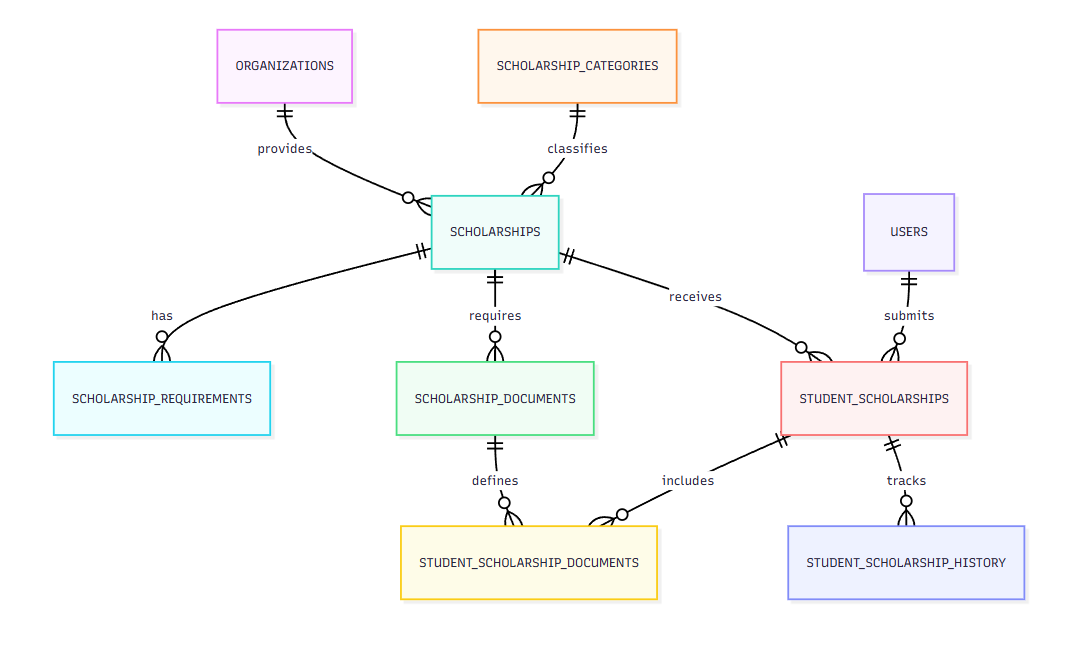
\includegraphics[width=0.9\textwidth]{images/chapter3/scholarship/scholarship-erd.png}%
    }{%
        \rectbox{Sơ đồ ERD cho phân hệ học bổng}
    }
    \caption{Sơ đồ ERD cho phân hệ học bổng}
    \label{fig:erd-scholarship}
\end{figure}

\section{Luồng tương tác giữa các thành phần}
Phần này mô tả ba luồng tương tác tiêu biểu giữa các thành phần kiến trúc, ở góc nhìn thành phần nào tham gia và giao tiếp qua kênh nào; đặc tả chi tiết từng bước nghiệp vụ và endpoint cụ thể của các luồng này được trình bày tại Chương 4.

\subsection{Luồng ghi nhận và phân loại giao dịch bằng AI}
Sinh viên nhập một mô tả giao dịch bằng ngôn ngữ tự nhiên trên Mobile App. Yêu cầu được gửi tới Backend qua HTTP REST; Backend chuyển tiếp sang AI Service để phân loại; AI Service trả về hũ tài chính và danh mục chi tiêu được đề xuất; Backend chuyển kết quả này về Mobile App để sinh viên xác nhận trước khi lưu giao dịch vào PostgreSQL.

\subsection{Luồng trò chuyện AI thời gian thực}
Sinh viên đặt câu hỏi trong màn hình trò chuyện AI. Mobile App mở một kết nối SSE tới Backend; Backend xác thực rồi chuyển tiếp yêu cầu sang AI Service; AI Service suy luận và truy vấn dữ liệu thật qua Backend khi cần, sau đó truyền câu trả lời về dưới dạng luồng token liên tục; Backend chuyển tiếp luồng này về Mobile App để hiển thị theo thời gian thực (Hình~\ref{fig:ai-flow}).

\subsection{Luồng xét duyệt học bổng và thông báo kết quả}
Nhà tài trợ cập nhật trạng thái một hồ sơ ứng tuyển trên Web Admin Portal. Yêu cầu được gửi tới Backend qua HTTP REST; Backend cập nhật trạng thái hồ sơ trong PostgreSQL, sau đó đẩy một tác vụ gửi thông báo vào hàng đợi Redis thay vì gửi ngay trong cùng yêu cầu; một worker chạy nền lấy tác vụ ra khỏi hàng đợi và gọi Firebase Cloud Messaging để gửi thông báo đẩy tới thiết bị của sinh viên.

\section{Đánh giá kiến trúc hệ thống}

\subsection{Ưu điểm}
Kiến trúc phân tán nhiều tầng, đa-repository giúp tách trách nhiệm rõ ràng theo cả chiều tầng (trình bày/ứng dụng/dữ liệu) lẫn chiều dịch vụ (Mobile, Web Admin, Backend, AI Service). Mỗi cặp thành viên trong nhóm có thể phát triển độc lập trên repository riêng của mình, hạn chế xung đột mã nguồn khi làm việc song song (liên kết với cách phân công tại Chương 5). Việc tách AI Service thành một dịch vụ riêng giúp cô lập hoàn toàn rủi ro về độ trễ, lỗi hoặc chi phí gọi mô hình ngôn ngữ lớn khỏi các nghiệp vụ lõi (tài chính, học bổng), đảm bảo các chức năng cốt lõi vẫn hoạt động ổn định ngay cả khi thành phần AI gặp sự cố. Việc xử lý bất đồng bộ qua hàng đợi giúp hệ thống chịu tải tốt khi cần gửi thông báo tới số lượng lớn người dùng cùng lúc mà không làm chậm các yêu cầu API chính.

\subsection{Khả năng mở rộng và bảo trì}
Kiến trúc phân lớp và module hóa theo miền nghiệp vụ cho phép bổ sung dịch vụ hoặc miền nghiệp vụ mới mà không phá vỡ cấu trúc hiện có. Tầng trừu tượng hóa nhà cung cấp mô hình ngôn ngữ lớn tại AI Service cho phép đổi hoặc bổ sung nhà cung cấp mới mà không cần sửa đổi logic nghiệp vụ ở các tầng phía trên. Việc tổ chức đa-repository, mỗi dịch vụ một repository riêng, giúp giảm xung đột mã nguồn giữa các nhóm nhỏ và cho phép mỗi dịch vụ được triển khai, phiên bản hóa độc lập với các dịch vụ còn lại.

\subsection{Hướng mở rộng kiến trúc trong tương lai}
Mã nguồn của AI Service hiện đã chuẩn bị sẵn một khung điều phối đa-agent (multi-agent orchestration), cho phép định tuyến yêu cầu tới nhiều tác nhân AI chuyên biệt theo từng miền nghiệp vụ khác nhau; tuy nhiên khung này chưa được kích hoạt trong luồng xử lý thực tế ở phiên bản hiện tại, mà chỉ mới sử dụng một tác nhân duy nhất với cơ chế phân loại ý định như đã mô tả ở Mục 3.4. Đây là nền tảng sẵn có để hệ thống có thể mở rộng thành kiến trúc đa-agent thực thụ khi bổ sung thêm các nghiệp vụ AI phức tạp hơn trong tương lai.

\subsection{Giới hạn hiện tại}
Nhìn từ góc độ kiến trúc, hệ thống còn một số giới hạn: một số thao tác tài chính tổng hợp (như phân bổ thu nhập vào nhiều hũ cùng lúc) chưa được bọc trong một transaction cơ sở dữ liệu tường minh, tiềm ẩn rủi ro không nhất quán nếu xảy ra lỗi giữa chừng (chi tiết tại Chương 4); hệ thống chưa có bộ benchmark định lượng chính thức, có thể tái lập cho các thành phần AI (chi tiết tại Chương 6); và hệ thống phụ thuộc vào các dịch vụ bên thứ ba nằm ngoài tầm kiểm soát trực tiếp (Firebase Cloud Messaging, nhà cung cấp mô hình ngôn ngữ lớn).
